\documentclass[12pt,letterpaper]{article}
\usepackage{fullpage}
\usepackage[top=2cm, bottom=4.5cm, left=2.5cm, right=2.5cm]{geometry}
\usepackage{amsmath,amsthm,amsfonts,amssymb,amscd}
\usepackage{lastpage}
\usepackage{enumerate}
\usepackage{fancyhdr}
\usepackage{mathrsfs}
\usepackage{xcolor}
\usepackage{graphicx}
\usepackage{listings}
\usepackage{hyperref}

\hypersetup{%
  colorlinks=true,
  linkcolor=blue,
  linkbordercolor={0 0 1}
}
 
\renewcommand\lstlistingname{Algorithm}
\renewcommand\lstlistlistingname{Algorithms}
\def\lstlistingautorefname{Alg.}

\lstdefinestyle{Python}{
    language        = Python,
    frame           = lines, 
    basicstyle      = \footnotesize,
    keywordstyle    = \color{blue},
    stringstyle     = \color{green},
    commentstyle    = \color{red}\ttfamily
}

\setlength{\parindent}{0.0in}
\setlength{\parskip}{0.05in}

\DeclareMathOperator{\Var}{Var}
\DeclareMathOperator{\Cov}{Cov}
\usepackage{multirow}
\usepackage{array}
\usepackage{tabularx}
\renewcommand{\arraystretch}{1.4}

% Edit these as appropriate
\newcommand\course{Econometrics, HSE}
\newcommand\testnumber{1}                  
\newcommand\testdate{October 1, 2021}

\pagestyle{fancyplain}
\headheight 35pt

\chead{\textbf{\Large Test \testnumber}}
\lhead{\testdate}
\rhead{\course}
\lfoot{}
\cfoot{}
\rfoot{\small\thepage}
\headsep 1.5em

\begin{document}

You have 40 minutes to complete the test. Please explain each step of your derivations and state all the assumptions employed. Note that different problems can give you different points. Maximum for the test is 10 points.  

\section*{Problem 1} 

Some practitioners of econometrics consider regressions with transformed variables. For example, if the original model specification is:
\begin{equation*}
    Y_i = \beta_1 + \beta_2 X_i + u_i
\end{equation*}

the revised specification is:
\begin{equation*}
    Y_i^* = \beta_1^* + \beta_2^* X_i^* + v_i
\end{equation*}

where:
\begin{equation*}
    Y_i^* = \frac{Y_i - a}{c} \quad\mbox{and}\quad X_i^* = 
    \frac{X_i - b}{d}.
\end{equation*}

Knowing that $a, b, c, d$ are some constants and $ c \ne 0, d \ne 0$, express the OLS estimators $\widehat\beta_1^*$, $\widehat\beta_2^*$ in terms of the OLS estimators $\widehat\beta_1$, $\widehat\beta_2$ [2 points].


\section*{Problem 2}
A novice econometrician estimated a classical linear model 
\begin{equation*}
     Y_i = \beta_1 + \beta_2 X_i + u_i
\end{equation*}

using 4 observations and obtained the following results:\\
\begin{table}[h]
\centering
\begin{tabularx}{0.6\textwidth} { 
  | >{\centering\arraybackslash}X 
  || >{\centering\arraybackslash}X 
  | >{\centering\arraybackslash}X 
  | >{\centering\arraybackslash}X 
  | >{\centering\arraybackslash}X | }
 \hline
 $Y_i$ & 3 & 7 & 9 & 10\\ 
 \hline
 $X_i$ & 3 & XXX & XXX & 1\\ 
  \hline
 $\widehat Y_i$ & 4 & 8 & 7 & 11\\ 
 \hline
\end{tabularx}
\end{table}

Help this econometrician find the estimates of the regression coefficients $\hat \beta_1$ and $\hat \beta_2$ [1 point] and restore the missing values in table [1 point]. Can you confirm that these estimations were made using the OLS method? [1 point]

\section*{Problem 3}
The output below gives the result of regressing $WAGE$, individual monthly wage measured in thousand rubles, on $TENURE$, total years of work experience a person has.

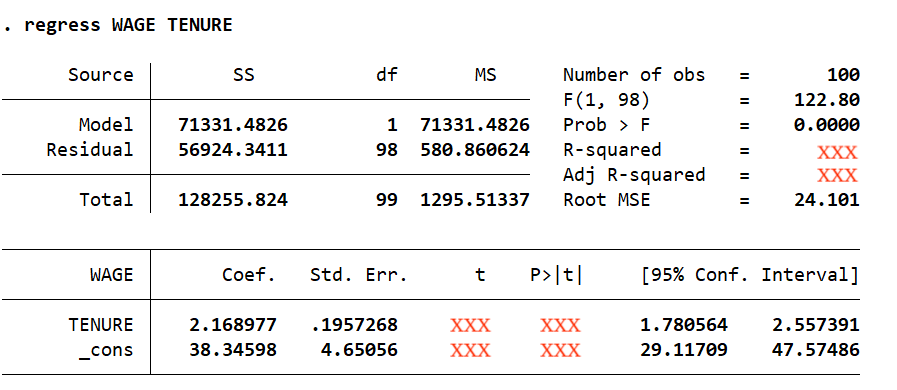
\includegraphics[scale=0.72]{Test1-model.png}

Unfortunately, some things are missing. Looking at this output, do the following tasks:

\begin{enumerate}
    \item 
    Give an interpretation of the coefficients estimations [1 point]
    
    \item
    Tell whether coefficients are statistically significant or not (if necessary, you may assume that these hypotheses are tested at a $5\%$ significance level, $t_{crit} \approx 2$) [1 point]
    
    \item
    Find the $R^2$ value [0.5 points]
    
    \item
    Explain in your own words what the $R^2$ value shows [0.5 points]
    
\end{enumerate}


\section*{Problem 4}
We have a linear model 
\begin{equation*}
    Y_i = \beta X_i + u_i
\end{equation*}

where $\beta$ is a fixed parameter, $u_i$ is a disturbance term that is independently and identically distributed with expected value 0 and population variance $\sigma_u^2$ and $i = {1, ..., n}$ is the observation index.

\setlength{\parskip}{1em} 
Derive the OLS  $\hat \beta$ estimator. Answers without a solution will not be accepted. You need to provide a full solution. [2 points]


\end{document}
